\documentclass[11pt,letterpaper]{article}
\usepackage[margin=.68in]{geometry}
\usepackage[T1]{fontenc}
\usepackage{lmodern,microtype,booktabs,array,graphicx,xcolor,amsmath,hyperref}
\hypersetup{colorlinks=true,urlcolor=blue,linkcolor=blue,pdftitle={Fiscal labels do not guarantee a better revenue forecast}}
\setlength{\parindent}{0pt}\setlength{\parskip}{6pt}
\newcommand{\heading}[1]{\vspace{4pt}{\large\bfseries #1}\par}
\newcommand{\BoundA}{4.758807}
\newcommand{\BoundB}{4.776929}
\newcommand{\BoundC}{373}
\newcommand{\BoundD}{7,007}
\newcommand{\BoundE}{71}
\newcommand{\BoundF}{62}
\newcommand{\BoundG}{6.789346}
\newcommand{\BoundH}{10.048371}
\newcommand{\BoundI}{71}
\newcommand{\BoundJ}{131}
\newcommand{\BoundK}{121}
\newcommand{\BoundL}{48}
\newcommand{\BoundM}{2}
\newcommand{\BoundN}{373}
\newcommand{\BoundO}{2024-02-03}
\newcommand{\BoundP}{0}
\newcommand{\BoundQ}{5}
\newcommand{\BoundR}{4}
\newcommand{\BoundS}{4}
\newcommand{\BoundT}{5}
\newcommand{\BoundU}{12.705400}
\newcommand{\BoundV}{13.820044}
\newcommand{\BoundW}{11.087482}
\newcommand{\BoundX}{5}
\newcommand{\BoundY}{4.037667}
\newcommand{\BoundZ}{4.318185}
\newcommand{\BoundAA}{3.799111}
\newcommand{\BoundAB}{5}
\newcommand{\BoundAC}{4.483902}
\newcommand{\BoundAD}{5.083163}
\newcommand{\BoundAE}{4.162288}
\newcommand{\BoundAF}{5}
\newcommand{\BoundAG}{4.537232}
\newcommand{\BoundAH}{5.284174}
\newcommand{\BoundAI}{4.179549}
\newcommand{\BoundAJ}{4}
\newcommand{\BoundAK}{11.189250}
\newcommand{\BoundAL}{11.328684}
\newcommand{\BoundAM}{14.266926}
\newcommand{\BoundAN}{4}
\newcommand{\BoundAO}{2.615641}
\newcommand{\BoundAP}{2.977488}
\newcommand{\BoundAQ}{3.260876}
\newcommand{\BoundAR}{4}
\newcommand{\BoundAS}{2.497164}
\newcommand{\BoundAT}{3.102052}
\newcommand{\BoundAU}{3.124745}
\newcommand{\BoundAV}{4}
\newcommand{\BoundAW}{2.556555}
\newcommand{\BoundAX}{2.784045}
\newcommand{\BoundAY}{3.220298}
\newcommand{\BoundAZ}{4}
\newcommand{\BoundBA}{8.373750}
\newcommand{\BoundBB}{8.837549}
\newcommand{\BoundBC}{4.790704}
\newcommand{\BoundBD}{4}
\newcommand{\BoundBE}{12.798273}
\newcommand{\BoundBF}{13.060187}
\newcommand{\BoundBG}{7.431864}
\newcommand{\BoundBH}{4}
\newcommand{\BoundBI}{12.173222}
\newcommand{\BoundBJ}{12.715744}
\newcommand{\BoundBK}{7.043753}
\newcommand{\BoundBL}{4}
\newcommand{\BoundBM}{11.838052}
\newcommand{\BoundBN}{12.404379}
\newcommand{\BoundBO}{6.876572}
\newcommand{\BoundBP}{13}
\newcommand{\BoundBQ}{10.756133}
\newcommand{\BoundBR}{11.509923}
\newcommand{\BoundBS}{10.048371}
\newcommand{\BoundBT}{13}
\newcommand{\BoundBU}{6.483860}
\newcommand{\BoundBV}{8.125692}
\newcommand{\BoundBW}{4.830617}
\newcommand{\BoundBX}{13}
\newcommand{\BoundBY}{6.384763}
\newcommand{\BoundBZ}{8.106611}
\newcommand{\BoundCA}{4.776929}
\newcommand{\BoundCB}{13}
\newcommand{\BoundCC}{6.310613}
\newcommand{\BoundCD}{7.948627}
\newcommand{\BoundCE}{4.758807}
\newcommand{\BoundCF}{373}
\newcommand{\BoundCG}{7,007}
\newcommand{\BoundCH}{38,426}
\newcommand{\BoundCI}{4,243}
\newcommand{\BoundCJ}{2}
\newcommand{\BoundCK}{2}
\newcommand{\BoundCL}{4}
\begin{document}
{\LARGE\bfseries Fiscal labels do not guarantee a better revenue forecast\par}
\vspace{5pt}Independent research program\hfill 31 October 2026 UTC\\
\textit{Not peer reviewed. Three-company, current-source retrospective reconstruction.}

\heading{Practical finding}
Pooling revenue growth by fiscal-quarter labels is a modeling choice to test. In the protected cohort, calendar pooling has a macro mean absolute percentage error (MAPE) of \BoundA{}\%, compared with \BoundB{}\% for fiscal pooling. The small ordering changes across company and year checks. This sample does not establish a general winner.

For a finance-data team, retain actual report intervals, accessions and filing-day availability before building a panel. Compare fiscal alignment with calendar grouping and a same-quarter baseline using information available at each origin. Do not choose the final model from the test scores shown here.

\heading{What was measured}
The target is next fiscal year's reported quarterly revenue for the same fiscal slot, conditional on that slot persisting. The source is exactly the SEC Company Facts USD concept \texttt{RevenueFromContract\allowbreak{}WithCustomer\allowbreak{}ExcludingAssessedTax}, joined to Submissions filing metadata for Apple, Microsoft and Walmart. No concept or company is replaced after inspection. Fourth-quarter residuals are not inferred.

The complete source projection contains \BoundC{} revenue entries and \BoundD{} filing metadata rows. Own-current-report matching, duration and fiscal-focus rules leave \BoundE{} observations and \BoundF{} prior-year pairs. All exclusions and unavailable prior slots remain in the public accounts.

\heading{A result that depends on the evaluation period}
The validation winner is the zero-growth same-quarter baseline, at \BoundG{}\% macro MAPE. Its protected-test MAPE is \BoundH{}\%. Both grouped families select zero shrinkage on validation. Their test scores improve over this baseline in the observed cohort, but this does not retrospectively change the committed validation choice.

\heading{Material limits}
This is a current-source filing-day reconstruction, not a verified immutable production point-in-time dataset. Three familiar companies and two target calendar years are too few independent blocks for calibrated confidence intervals, significance claims or market-wide recommendations. There is no investment, causal, adoption, new-estimator or realized-savings claim.

\newpage
\heading{Source identity and complete observation accounting}
Eight decoded native public JSON responses were captured on 31 October 2026 UTC. SHA-256, size, exact endpoint, retrieval time and transport controls are retained. Earlier command-line access was denied; an ordinary browser navigation returned public data. Raw JSON and corporate labels, prose and contact fields remain private. The public subset contains minimal numerical, period and filing identifiers with attribution.

An entry must be an original 10-Q whose accession has unique, consistent Submissions metadata. Its source form and filed day must match. Its end must equal that filing's own reportDate. This prevents the current filing's fiscal focus from being assigned to a comparative prior period. The interval must span 61--121 inclusive days; fiscal focus must be Q1, Q2 or Q3; fiscal year must be known; USD revenue must be finite and positive.

\begin{center}\begin{tabular}{lr}\toprule
Complete revenue-entry account & Entries\\\midrule
Selected observations & \BoundI{}\\
Not original 10-Q & \BoundJ{}\\
Comparative or noncurrent end & \BoundK{}\\
Not quarterly duration & \BoundL{}\\
Outside fixed observation window & \BoundM{}\\\midrule
All entries & \BoundN{}\\\bottomrule\end{tabular}\end{center}
Exact repeats retain multiplicity. Conflicting economic contexts or fiscal-slot report ends make an observation unavailable. If multiple original accessions share a consistent slot/end, the earliest filed day then accession is selected. The observed cohort needs no conflicting-context exclusions; the code still rejects those cases. Missingness is never converted to zero.

\heading{Origin, label availability and temporal protection}
Observation ends are fixed to 2018--June 2026. Pair a target with the same company's previous fiscal-year focus and quarter, requiring a 335--395-day end-date gap. The origin is the prior filing day plus one calendar day. Inputs are its reported amount, known fiscal quarter and actual prior end's calendar quarter. A target growth label becomes available one day after its own filed day; fitting requires availability strictly before the origin. Future target dates and focus are not input features.

Training uses Apple/Microsoft labels with report ends in 2019--2021. Validation uses their 2022--2023 targets. Test fitting may use their labels through 2023, still availability filtered. All 2024 growth labels are embargoed; already reported 2024 amounts can be prior inputs. Walmart growth labels never fit or select. Every protected test origin follows the validation-label closure of \BoundO{}. Actual source/evaluation minimums pass without changing dates or companies.

\newpage
\heading{Methods, baselines and validation selection}
Let $R_i^-$ be prior same-slot revenue, $R_i$ the target and $g_i=R_i/R_i^- -1$. At origin $o$, fitting rows are the fixed training-company/window pairs with label availability strictly before $o$. Let $\bar g_o$ be their mean and $G_o(z)$ the rows with group $z$. The grouped forecast is
\[
 \hat R_i=R_i^-\left(1+\frac{\sum_{j\in G_o(z_i)}g_j+a\bar g_o}{|G_o(z_i)|+a}\right).
\]
Fiscal grouping uses known prior Q1/Q2/Q3. Calendar grouping uses the calendar quarter of the prior actual end. An unseen group falls back to the global mean, including at $a=0$. The authored pseudo-count grid is $a\in\{0,1,4,16\}$, a coarse range from no shrinkage to substantial pooling. It is not a globally optimized search. Positive inputs and convex mean growth preserve positive forecasts without clipping.

Two further baselines use zero growth and global mean growth. All ten validation candidates are retained. Primary selection first averages absolute percentage loss within company and then averages the two company means. This prevents the larger company or denser coverage from automatically dominating. Ties use smaller group strength; the overall tie order is zero, global, fiscal ascending strength, then calendar ascending strength. These are deterministic calculations without a random seed.

\begin{center}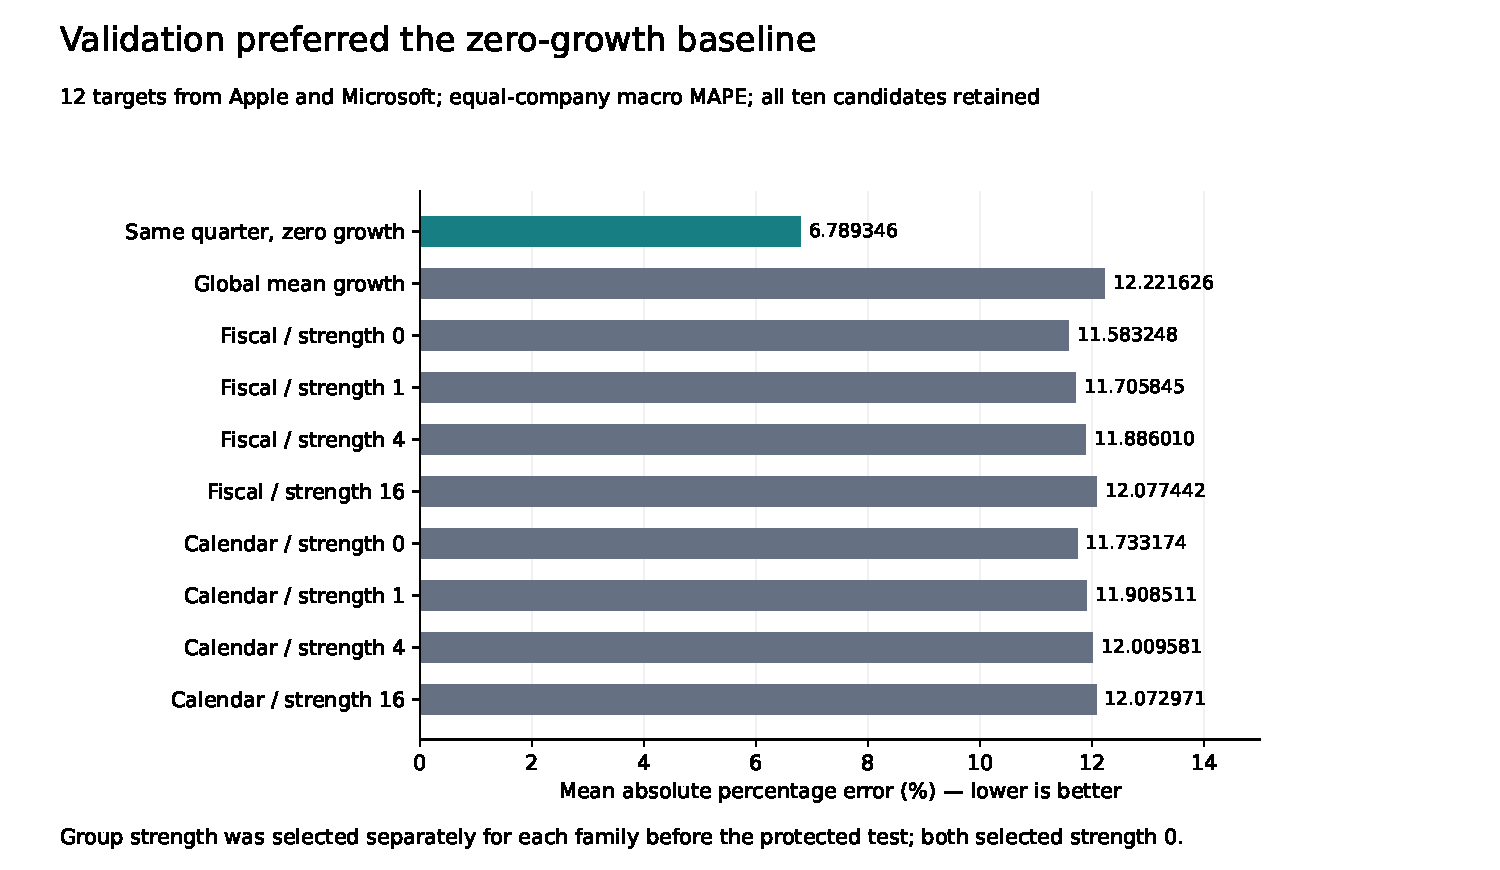
\includegraphics[width=\linewidth]{images/validation_candidates.pdf}\end{center}
Both selected group strengths are \BoundP{}. The validation configuration and prediction/metric hashes were committed before the first final-test command. Test evaluates exactly zero, global, selected fiscal and selected calendar. It is not reused to select another strength. Simple same-season forecasts and temporal evaluation are established methods; this contribution is a finite, reproducible calendar-feature comparison with explicit source and availability accounts [2].

\newpage
\heading{All protected-test company and macro results}
The fixed test window covers report ends in 2025--June 2026: Apple has \BoundQ{}, Microsoft \BoundR{} and held-out Walmart \BoundS{} pairs. No Walmart growth label enters training, validation or selection. Its own reported prior amount and known period labels are forecast inputs.

\begin{center}\small\begin{tabular}{llrrrr}\toprule
Company & Model & $n$ & MAE (USD bn) & RMSE (USD bn) & MAPE (\%)\\\midrule
Apple & Zero & \BoundT{} & \BoundU{} & \BoundV{} & \BoundW{}\\
Apple & Global & \BoundX{} & \BoundY{} & \BoundZ{} & \BoundAA{}\\
Apple & Fiscal / 0 & \BoundAB{} & \BoundAC{} & \BoundAD{} & \BoundAE{}\\
Apple & Calendar / 0 & \BoundAF{} & \BoundAG{} & \BoundAH{} & \BoundAI{}\\
\midrule
Microsoft & Zero & \BoundAJ{} & \BoundAK{} & \BoundAL{} & \BoundAM{}\\
Microsoft & Global & \BoundAN{} & \BoundAO{} & \BoundAP{} & \BoundAQ{}\\
Microsoft & Fiscal / 0 & \BoundAR{} & \BoundAS{} & \BoundAT{} & \BoundAU{}\\
Microsoft & Calendar / 0 & \BoundAV{} & \BoundAW{} & \BoundAX{} & \BoundAY{}\\
\midrule
Walmart & Zero & \BoundAZ{} & \BoundBA{} & \BoundBB{} & \BoundBC{}\\
Walmart & Global & \BoundBD{} & \BoundBE{} & \BoundBF{} & \BoundBG{}\\
Walmart & Fiscal / 0 & \BoundBH{} & \BoundBI{} & \BoundBJ{} & \BoundBK{}\\
Walmart & Calendar / 0 & \BoundBL{} & \BoundBM{} & \BoundBN{} & \BoundBO{}\\
\midrule
Macro & Zero & \BoundBP{} & \BoundBQ{} & \BoundBR{} & \BoundBS{}\\
Macro & Global & \BoundBT{} & \BoundBU{} & \BoundBV{} & \BoundBW{}\\
Macro & Fiscal / 0 & \BoundBX{} & \BoundBY{} & \BoundBZ{} & \BoundCA{}\\
Macro & Calendar / 0 & \BoundCB{} & \BoundCC{} & \BoundCD{} & \BoundCE{}\\
\bottomrule\end{tabular}\end{center}
MAE and MSE are exact rational means of USD errors and squared errors. MAPE divides by strictly positive actual revenue. RMSE is a 60-digit Decimal square root displayed to six decimals using half-even rounding. Public CSVs retain exact sums, MSE in USD squared and all original-scale displays. This table scales USD to billions for readability.

Macro MAE, MSE and MAPE are equal-company means of company metrics. Macro RMSE is the square root of macro MSE, rather than a mean of company RMSEs. The macro $n$ column is the total observed pair count, not the loss weighting rule.

Fiscal pooling slightly improves on calendar pooling for Apple and Microsoft; Walmart favors calendar pooling. Walmart's zero-growth baseline beats all growth-pooling candidates on its own four targets. This is a useful warning about transporting growth from two technology firms into a retailer, not evidence that an industry-specific replacement would pass a new untouched test.

The test forecasts and exact fitting-row memberships are retained for every candidate and target. Current numeric agreement verifies the reconstruction and arithmetic; it does not verify original-time publication, harmonize accounting policies or establish economic revenue truth.

\newpage
\heading{Company variation and descriptive dependence checks}
\begin{center}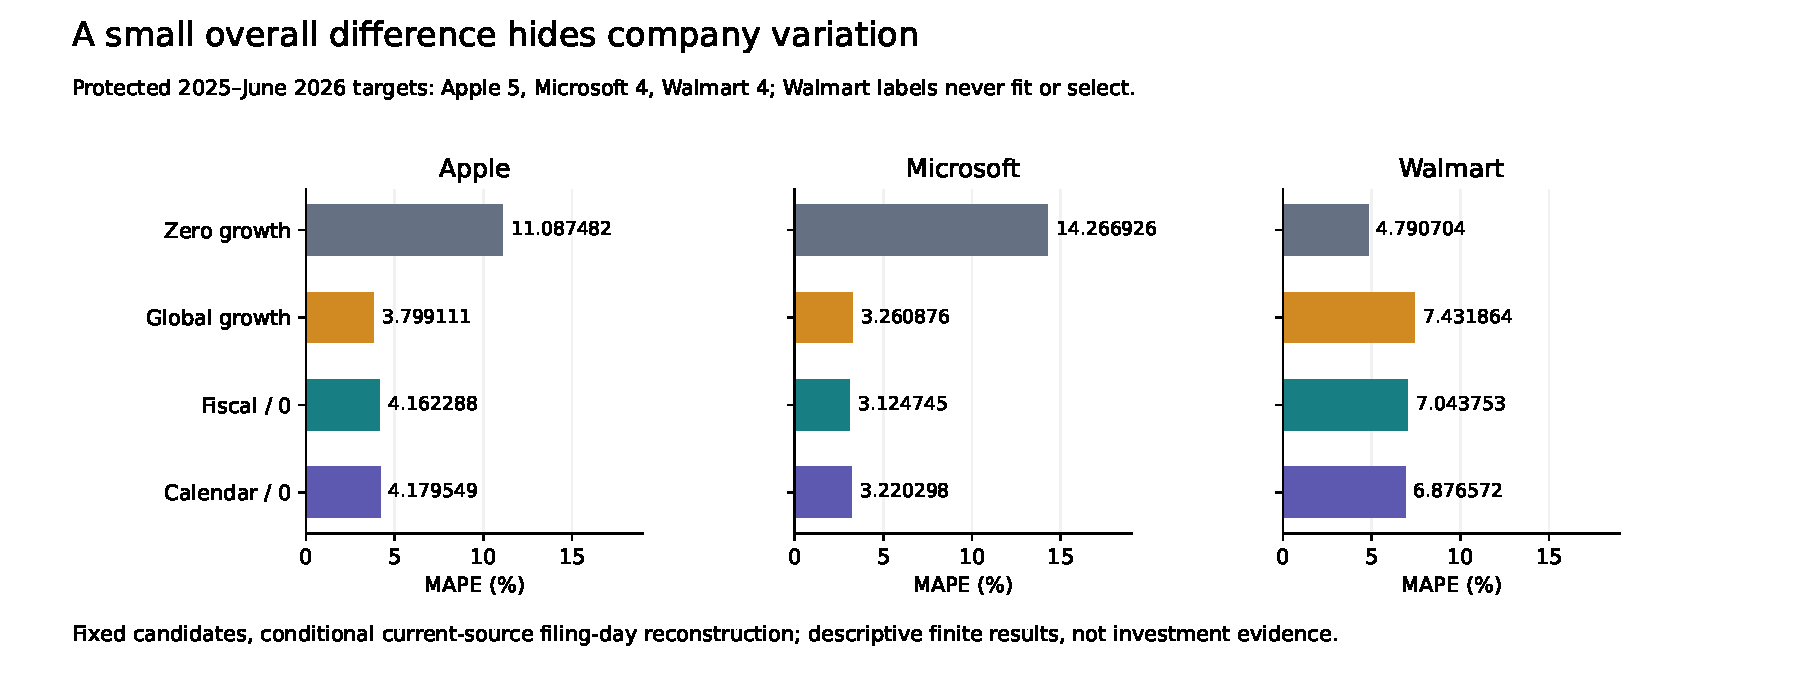
\includegraphics[width=\linewidth]{images/company_test.pdf}\end{center}
\begin{center}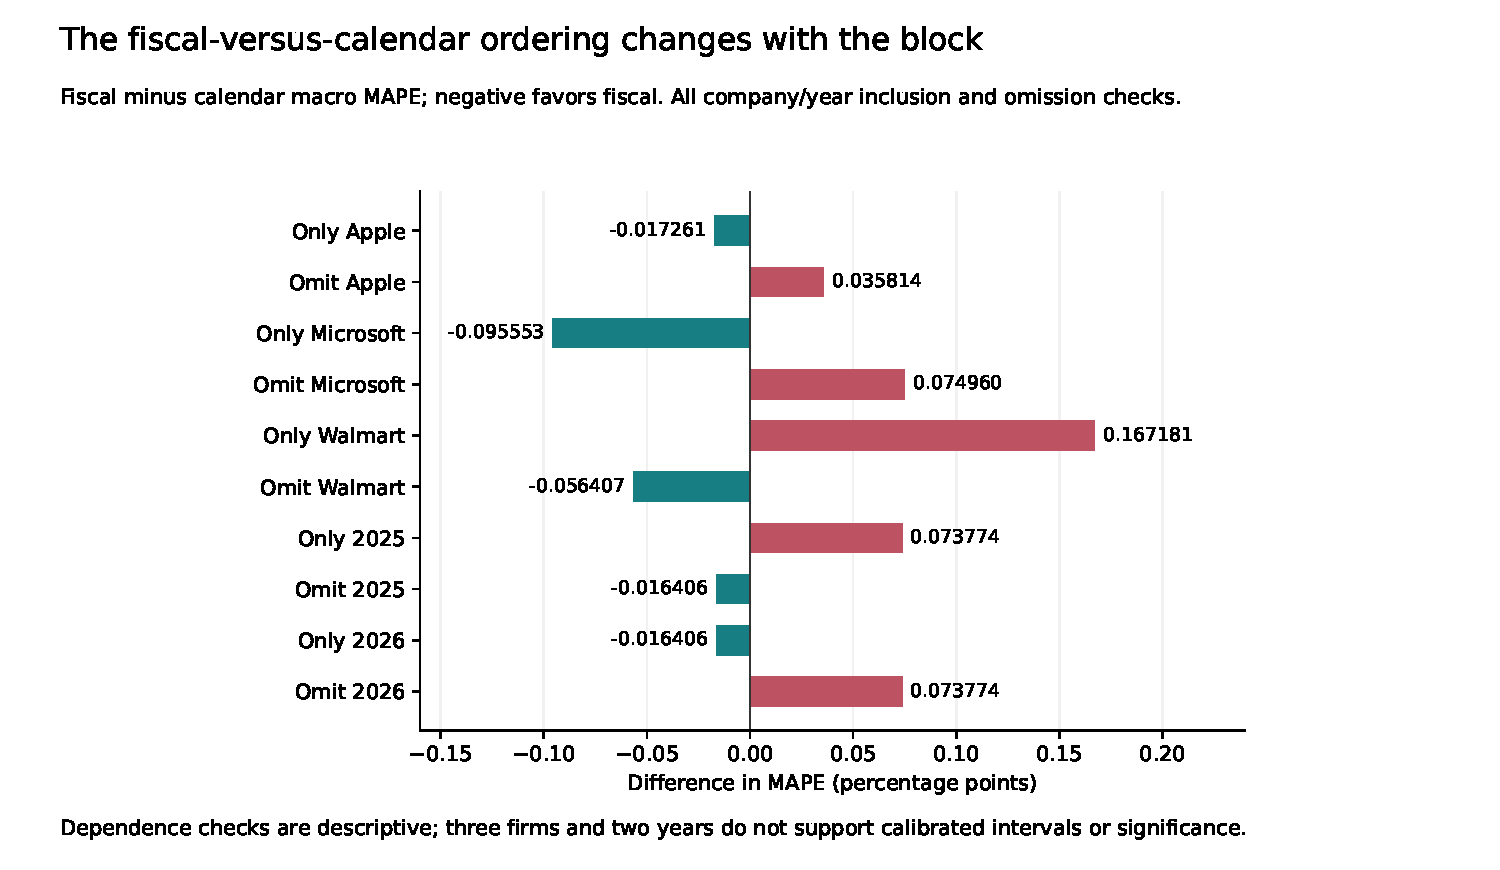
\includegraphics[width=.96\linewidth]{images/dependence_checks.pdf}\end{center}
Every paired fiscal-minus-calendar percentage loss is retained. All company-only, year-only, leave-one-company-out and leave-one-year-out macro differences are shown. Removing Walmart favors fiscal pooling; removing either training company favors calendar pooling. Calendar pooling is favored in the 2025 subset and fiscal pooling in the 2026 subset. These small changes are descriptive dependence checks. They are not confidence intervals, significance tests or independent randomized replications.

\newpage
\heading{Independent checks and reproducibility}
The native JSON check independently reconciles all eight hashes/bodies, \BoundCF{} exact revenue entries and \BoundCG{} metadata rows using \BoundCH{} finite conditions. A separate SQLite and Fraction checker reconstructs source exclusions, observation and pair identity, every available fitting set, all ten validation candidates, selection, four test models, metrics and dependence accounts without importing production model functions. Its final full-account check passes \BoundCI{} conditions. All 32 authored boundary fixture methods pass.

The actual source/method freeze binds 26 dependencies before validation. The selected configuration and validation files are committed at \texttt{771dfdb4c9a45fad55bc826be633f5ec13c1716d} before protected-test execution. No post-test source, method, strength or primary-output amendment is made. Separate full-history CPython 3.10.11 and 3.12.14 replays reproduce all 14 primary files byte for byte, leaving all six source-directory files unchanged each. Replay is of saved minimal data, not a new source acquisition or independent historical vintage.

\heading{Implementation exercise}
Run \texttt{python src/replay.py --out ../calendar-replay} after installing pinned requirements. The saved exercise accepts a complete reported-fiscal-slot/origin contract or abstains when the slot or origin is unavailable. Of eight requests, \BoundCJ{} return qualified forecasts, \BoundCK{} abstain and \BoundCL{} reject unsupported claims or fields. Investment advice, source-truth certification, exact future filing dates and arbitrary caller-data certification are outside the contract.

\heading{What further evidence would change the recommendation}
Use original-vintage dissemination records, more companies and sectors, complete fiscal years and more independent target periods before a production recommendation. The cohort omits Q4 and cases failing duration/metadata rules. It uses a single standardized concept and does not adjust for acquisitions, accounting changes, currency effects or alternate measures. The filing-day-plus-one rule is conservative at day resolution but does not recover exact timestamp availability. Current source revisions remain possible. No exhaustive scientific-priority claim is made.

\heading{Sources and publication boundary}
[1] U.S. Securities and Exchange Commission. \href{https://www.sec.gov/search-filings/edgar-application-programming-interfaces}{EDGAR Application Programming Interfaces}, current Company Facts/Submissions documentation. Exact eight source endpoints, decoded-body hashes and times are in \texttt{data/capture\_manifest.json}; minimal projections and complete accounts are public. Native JSON, corporate prose, labels, addresses, phone numbers, EINs and credentials remain private. MIT covers original code, not blanket rights in third-party expressive filings. No SEC endorsement.

[2] Hyndman, R.J. and Athanasopoulos, G. \textit{Forecasting: Principles and Practice}, third edition. \href{https://otexts.com/fpp3/toolbox.html}{The forecaster's toolbox}: simple benchmarks and forecast evaluation. Established methods motivate baselines; this study's company cohort, pooling grid, availability tolerance and temporal embargo are authored choices.

Independent-program manuscript authorized for public GitHub release. It is not peer reviewed or a formal submission. Separate formal-publication projects, including Azure optimization, remain private.
\end{document}
